\documentclass{article}
\usepackage{luatextra}
\usepackage{polyglossia}
\usepackage{ulem}
\usepackage{framed}
\usepackage{color}
\usepackage{geometry}
\usepackage{amsmath}
\usepackage{unicode-math}
\usepackage[hidelinks]{hyperref}
\usepackage{latexsym}
\usepackage{pdflscape}
\usepackage{pdfpages}
\usepackage{enumitem}
\usepackage{titlesec}
\usepackage{lastpage}
\usepackage{fancyhdr}

\usepackage{ifluatex}
\ifluatex
  \usepackage{pdftexcmds}
  \makeatletter
  \let\pdfstrcmp\pdf@strcmp
  \let\pdffilemoddate\pdf@filemoddate
  \makeatother
\fi
\usepackage{svg}


\setmainlanguage{french}
\selectlanguage{french}
\setdefaultlanguage{french}
%%\setmainfont{Latin Modern Roman}
\setmainfont{Roboto}

\geometry{margin={1in,1in}}


\setlist{nosep} %% No space between lists' items

\pagestyle{fancy}
\fancyhead[R]{}

%% <current page>/<total pages> footer
\cfoot{\thepage/\pageref{LastPage}}

\newcommand\image[2]{
\directlua{
local image = img.scan({filename = "#1"})

image.height = image.height * #2
image.width  = image.width  * #2

node.write(img.node(image))
}
}


%%%%%%%%%%%%%%%%%%%%%%%%%%%%%%%%%%%%%%%%%%
%% \subsubsubsection command definition %%
%%%%%%%%%%%%%%%%%%%%%%%%%%%%%%%%%%%%%%%%%%


\titleclass{\subsubsubsection}{straight}[\subsection]

\newcounter{subsubsubsection}[subsubsection]
\renewcommand\thesubsubsubsection{\thesubsubsection.\arabic{subsubsubsection}}
\renewcommand\theparagraph{\thesubsubsubsection.\arabic{paragraph}} % optional; useful if paragraphs are to be numbered

\titleformat{\subsubsubsection}
  {\normalfont\normalsize\bfseries}{\thesubsubsubsection}{1em}{}
\titlespacing*{\subsubsubsection}
{0pt}{3.25ex plus 1ex minus .2ex}{1.5ex plus .2ex}

\makeatletter
\renewcommand\paragraph{\@startsection{paragraph}{5}{\z@}%
  {3.25ex \@plus1ex \@minus.2ex}%
  {-1em}%
  {\normalfont\normalsize\bfseries}}
\renewcommand\subparagraph{\@startsection{subparagraph}{6}{\parindent}%
  {3.25ex \@plus1ex \@minus .2ex}%
  {-1em}%
  {\normalfont\normalsize\bfseries}}
\def\toclevel@subsubsubsection{4}
\def\toclevel@paragraph{5}
\def\toclevel@paragraph{6}
\def\l@subsubsubsection{\@dottedtocline{4}{7em}{4em}}
\def\l@paragraph{\@dottedtocline{5}{10em}{5em}}
\def\l@subparagraph{\@dottedtocline{6}{14em}{6em}}
\makeatother

\setcounter{secnumdepth}{4}
\setcounter{tocdepth}{4}

%%%%%%%%%%%%%%%%%%%%%%%%%%%%%%%%%%%%%%%%%%
%% end \subsubsubsection definition     %%
%%%%%%%%%%%%%%%%%%%%%%%%%%%%%%%%%%%%%%%%%%

\title{COO — Équipe 6}
\author{Cancela Joël\\Bounouas Nassim\\Mortara Johann\\Novac Pierre-Emmanuel}


\begin{document}
% a

\maketitle
\tableofcontents


\newpage
\section{Choix de conception}

\paragraph{}
La classe \texttt{Livre} représente une édition de livre alors qu'un exemplaire est un livre physique présent dans la bibliothèque. Cette relation est representée comme une association entre la classe \texttt{Livre} et la classe \texttt{Exemplaire de livre}. Un exemplaire n'est relié qu'à un seul livre mais un livre est relié à plusieurs exemplaires. Nous disposons d'un attribut calculé au sein du livre afin de connaitre le nombre d'exemplaires de ce livre présent dans la bibliothèque. La cote d'un exemplaire est representée par le numéro de document dont \texttt{Exemplaire de livre} hérite. Les détails concernant l'emprunt et  la réservation se retrouvent dans les classes d'associations \texttt{Emprunt} et \texttt{Réservation}.La perte se retrouve directement au sein de l'exemplaire. La méthode \texttt{est\_disponible()} de la classe exemplaire prend en considération les réservations, l'emprunt et la perte de l'exemplaire du livre.

\paragraph{}
La raison principale de ce choix de modélisation est principalement dû à l'emprunt, car on emprunte un exemplaire de livre mais il est nécessaire de connaitre le nombre d'exemplaires disponibles ou total pour un livre et la responsabilité n'est pas à un exemplaire de connaître les autres exemplaires.

\paragraph{}
Pour la gestion du temps, l'envoi des relances se fait chaque semaine passée le délai de rendu de l'emprunt au Lundi minuit. Nous considérons que notre système a la capacité de connaitre la date courante sans faire appel à une horloge externe.


\paragraph{}
La classe \texttt{Emprunt} contient la date et le nombre de relances pour celui-ci, la relance étant gérée par le serveur de messages nous avons choisi de ne pas modéliser de classe Relance, mais de préciser ses opérations dans le diagramme de séquence "Relancer pour rendu du livre".


\section{Diagramme de cas d'utilisation}

\vspace{-5em}
\hspace*{-8em}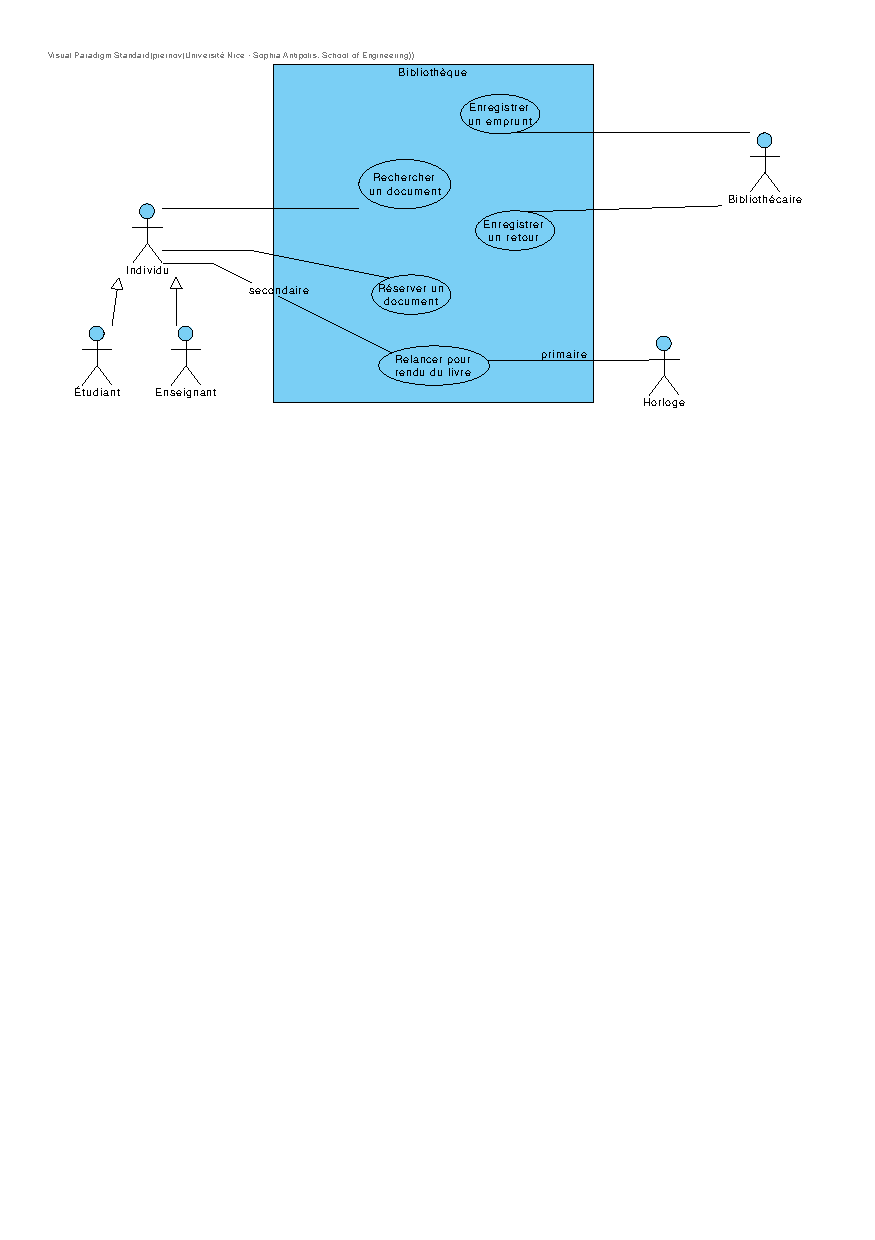
\includegraphics[scale=1.5]{use_case}
\vspace*{-4em}

\section{Cas d'utilisation: Enregistrer un emprunt}

\noindent\textbf{Nom:} Enregistrer un emprunt \\
\textbf{Description:} Un individu souhaite emprunter un livre.\\
\textbf{Précondition:} \\
\textbf{Postcondition:} Le livre est emprunté.\\
\textbf{Cas d'erreur:} Le livre n’existe pas, le livre est déjà emprunté, l’individu n’existe pas, l’individu est suspendu ou l’individu a déjà emprunté 3 livres.\\
\textbf{État du système en cas d'erreur:} L’emprunt n'est pas validé.\\
\textbf{Acteurs:} La bibliothécaire \\
\textbf{Déclenchement:} La bibliothécaire reçoit une demande d'emprunt d'un livre de la part d'un individu.\\
\textbf{Scénario primaire:}
\begin{enumerate}
	\item La bibliothécaire entre le numéro du document et le numéro de l'individu dans l'interface de la Bibliothèque.
	\item[1] La Bibliothèque recherche l'individu dans l'Annuaire.
	\item[2] La Bibliothèque recherche le livre dans le Fonds de bibliothèque.
	\item[3] Le livre est disponible, l'étudiant n'est pas suspendu et a moins de 3 emprunts.
	\item[4] La Bibliothèque enregistre l'emprunt.
\end{enumerate}

\noindent\textbf{Scénario alternatif:}
\begin{itemize}
	\item[2'.] L’étudiant n’existe pas, fin du cas d’utilisation.
	\item[3'.] Le livre n’existe pas, fin du cas d’utilisation.
	\item[4'.] Le livre est déjà emprunté, l’individu est suspendu ou l’individu a déjà emprunté 3 livres, fin du cas d’utilisation.
\end{itemize}


\section{Diagramme de classes}

\vspace{-5em}
\hspace*{-10em}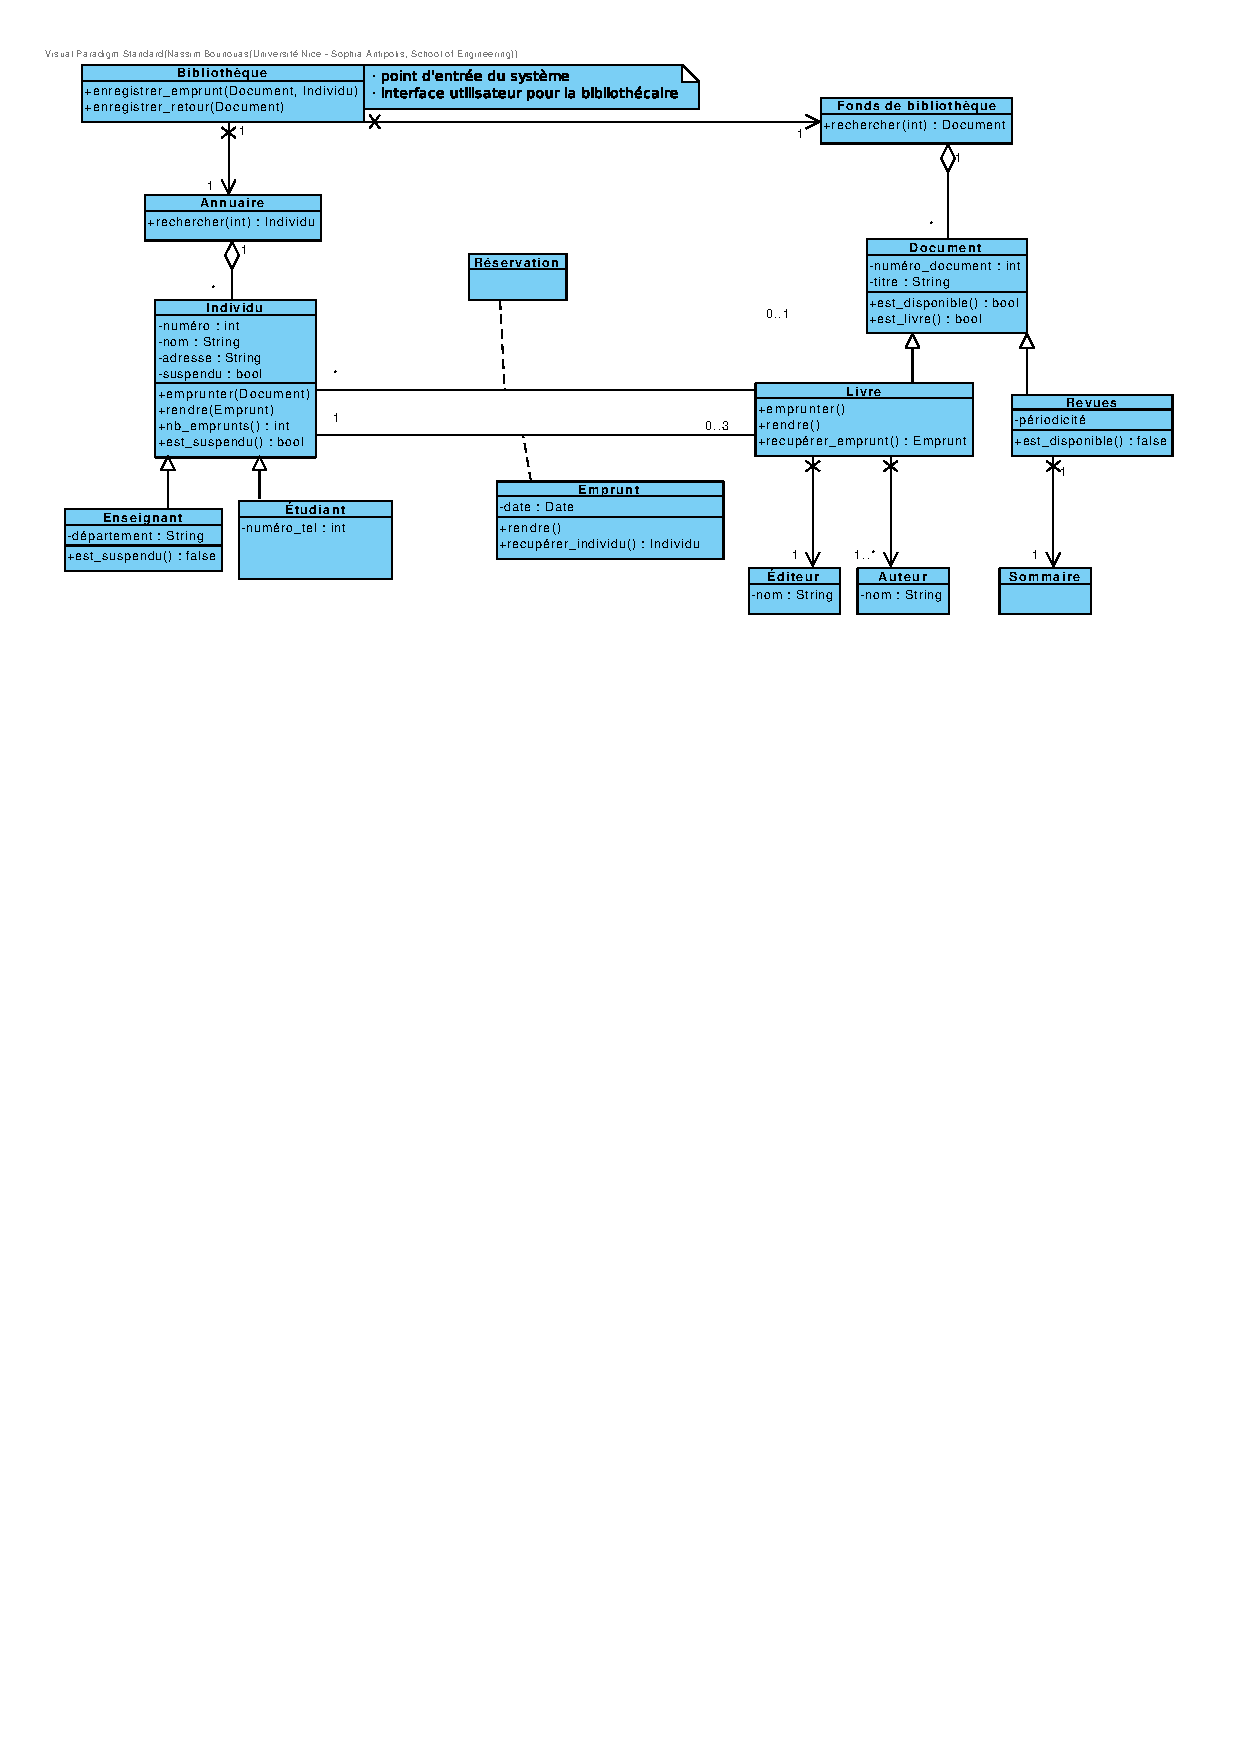
\includegraphics[scale=1.56]{class}
\vspace*{-4em}

\section{Diagrammes de séquence}

\subsection{Enregistrer un emprunt}
\vspace{-5em}
\hspace*{-10em}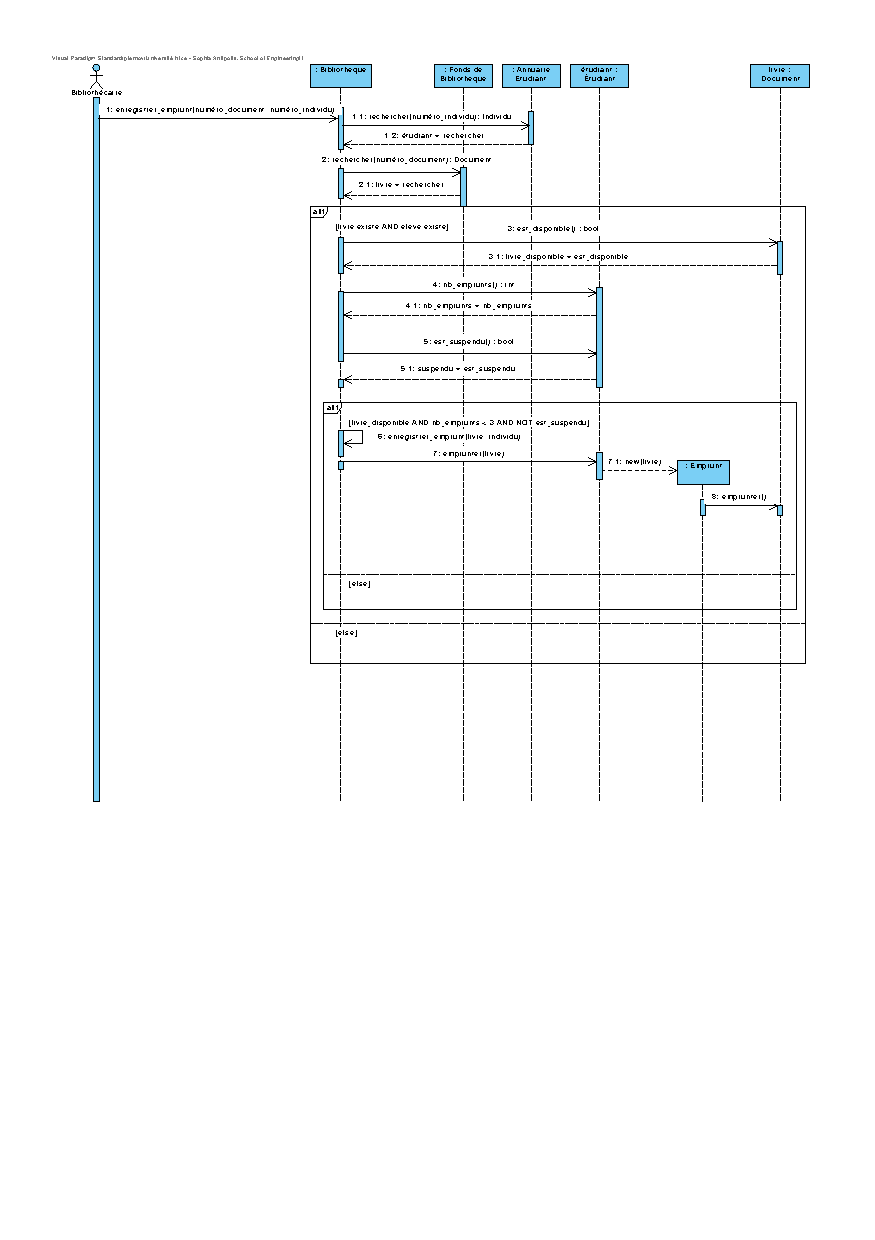
\includegraphics[scale=1.56]{sequence_enregistrer_un_emprunt}
\vspace*{-4em}

\subsection{Enregistrer un retour}
\vspace{-4em}
\hspace*{-9em}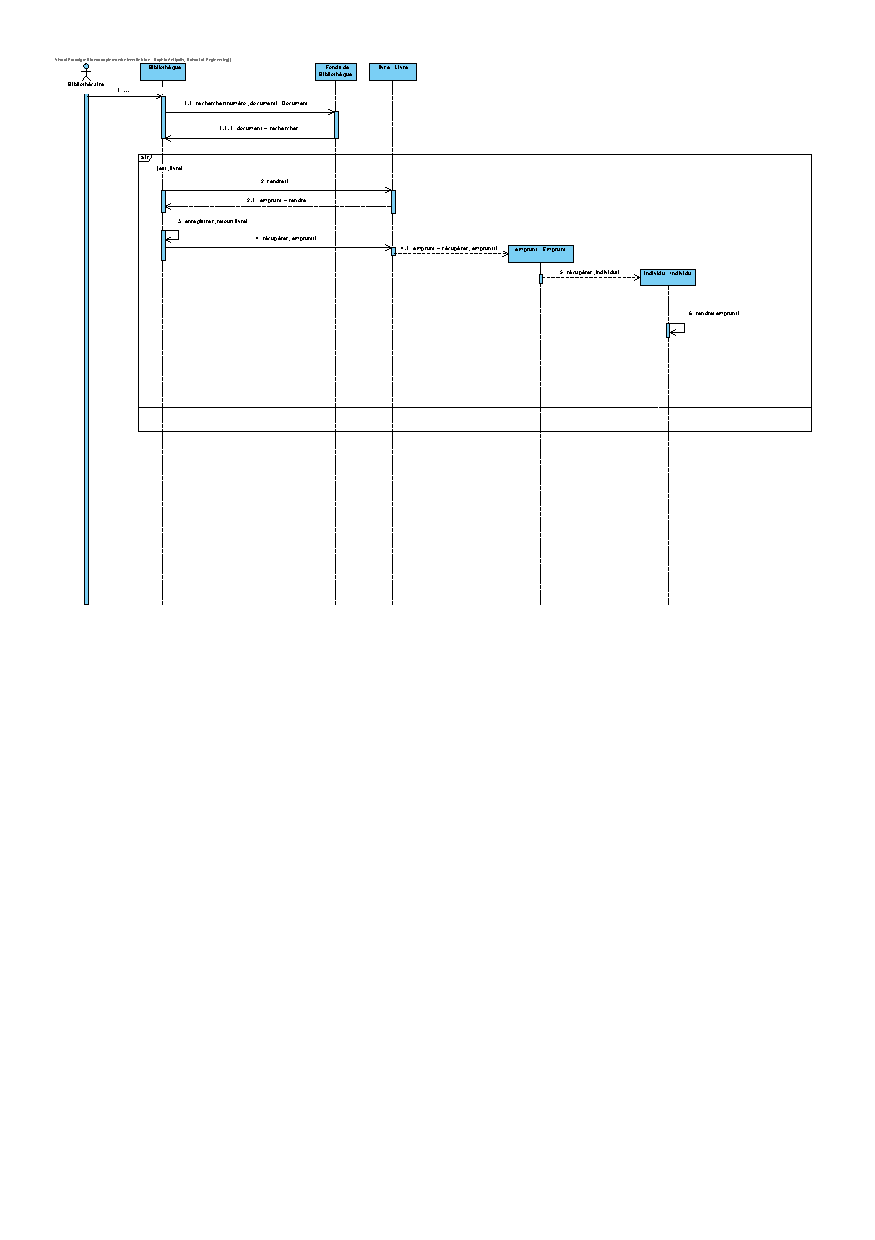
\includegraphics[scale=1.5]{sequence_enregistrer_un_retour}
\vspace*{-4em}

\subsection{Rechercher un document}
\vspace{-4em}
\hspace*{-9em}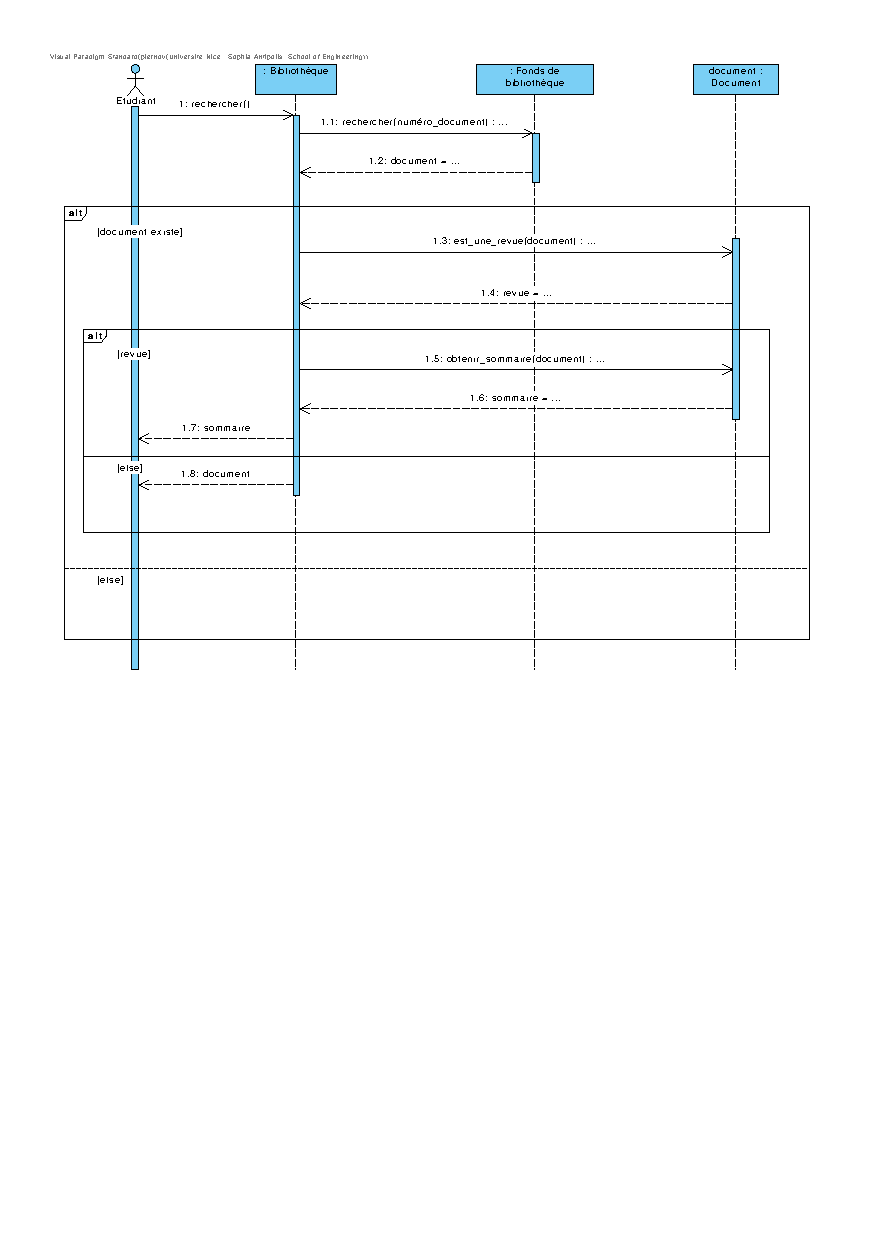
\includegraphics[scale=1.5]{sequence_rechercher_un_document}
\vspace*{-4em}

\subsection{Réserver un livre}
\vspace{-5em}
\hspace*{-10em}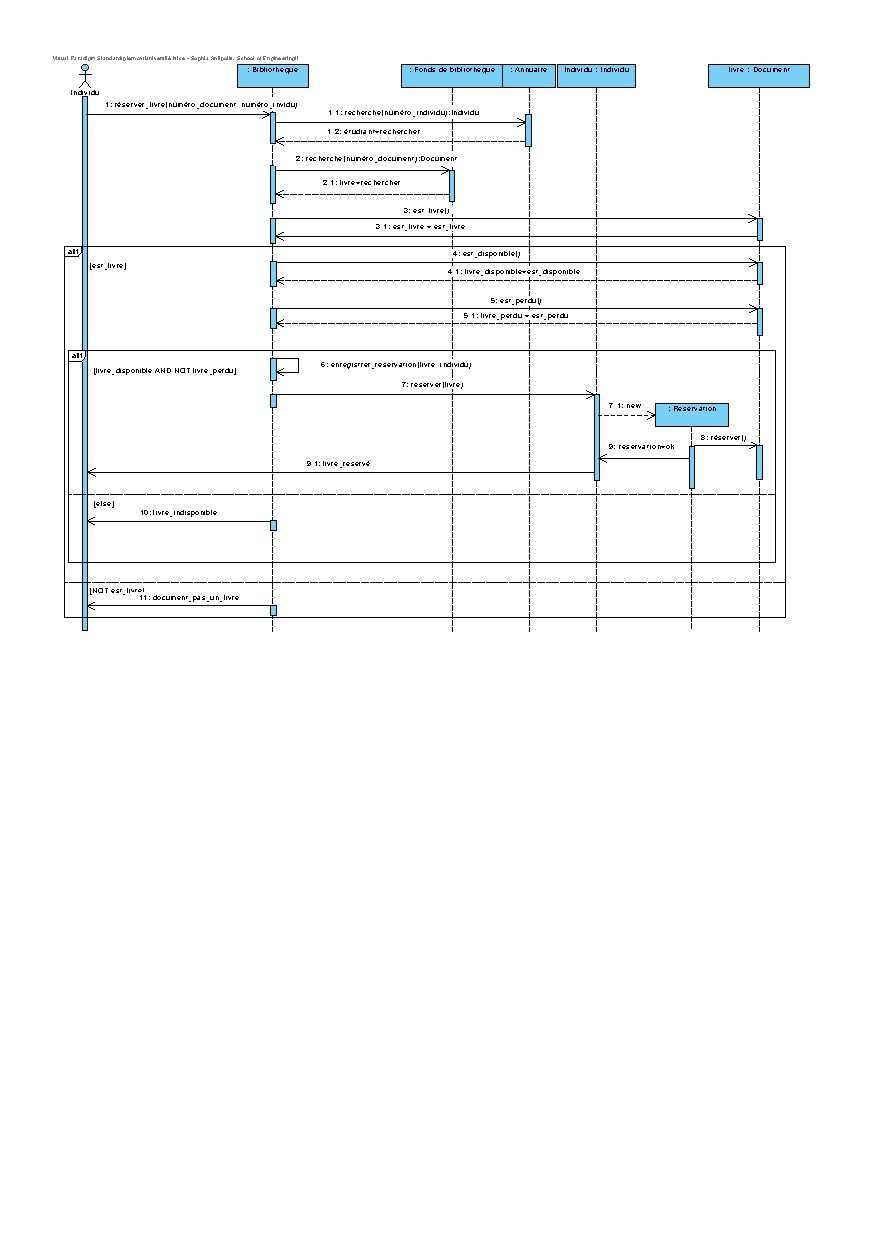
\includegraphics[scale=1.56]{sequence_reserver_un_livre}
\vspace*{-4em}

\subsection{Relancer pour rendu du livre}
\vspace{-4em}
\hspace*{-9em}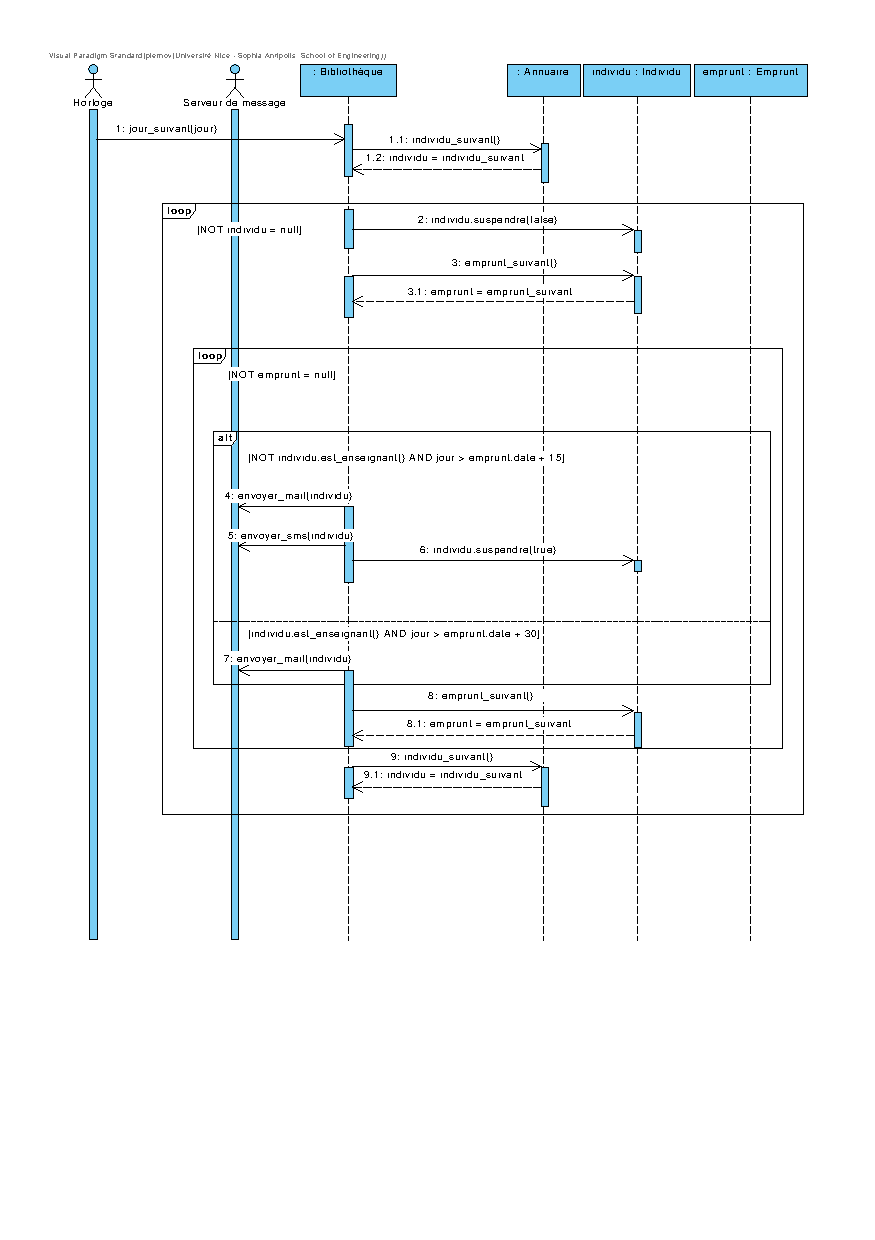
\includegraphics[scale=1.5]{sequence_relancer_pour_rendu_du_livre}
\vspace*{-4em}


\section{Diagrammes d'état}

\subsection{Exemplaire de Livre}
\vspace{-4em}
\hspace*{-9em}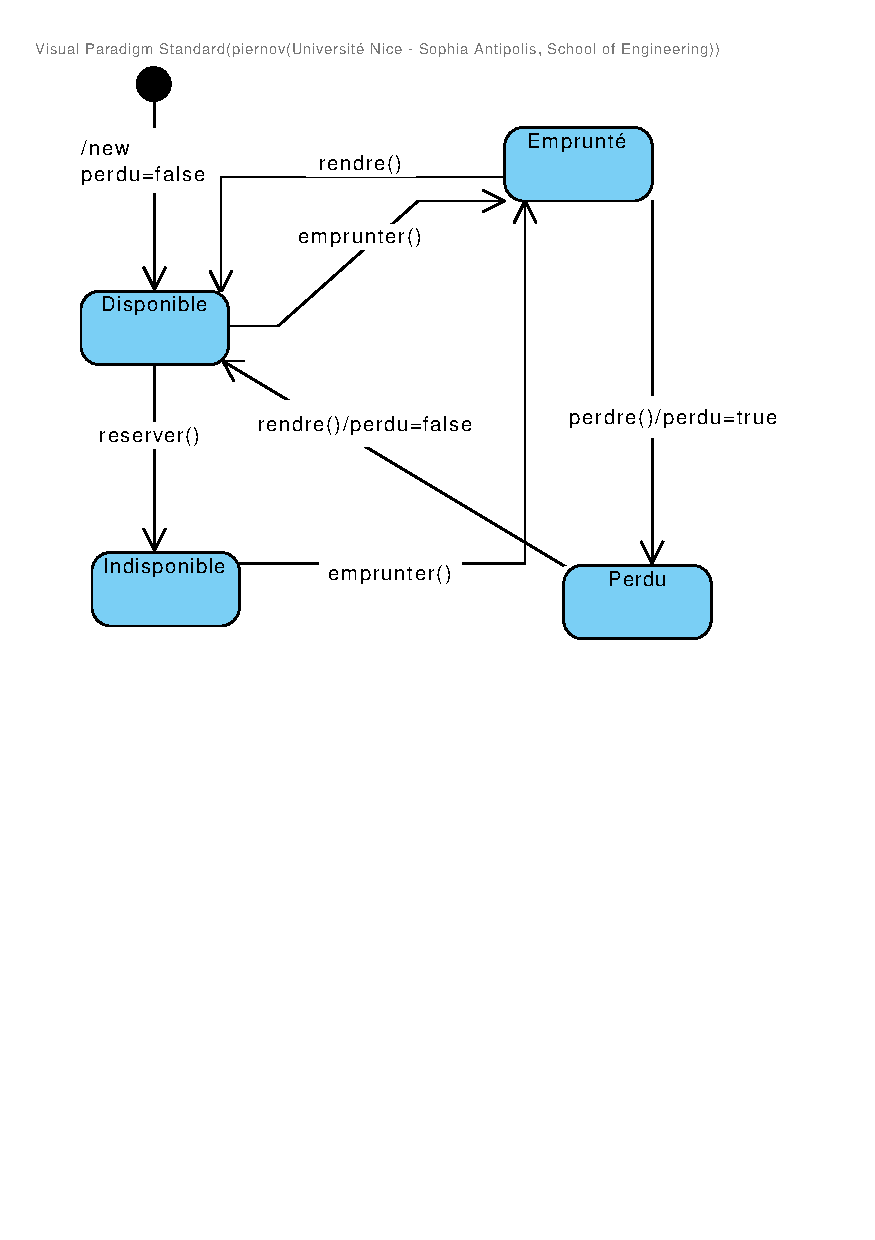
\includegraphics[scale=1.5]{state_exemplaire_de_livre}
\vspace*{-4em}

\subsection{Individu}
\vspace{-4em}
\hspace*{-9em}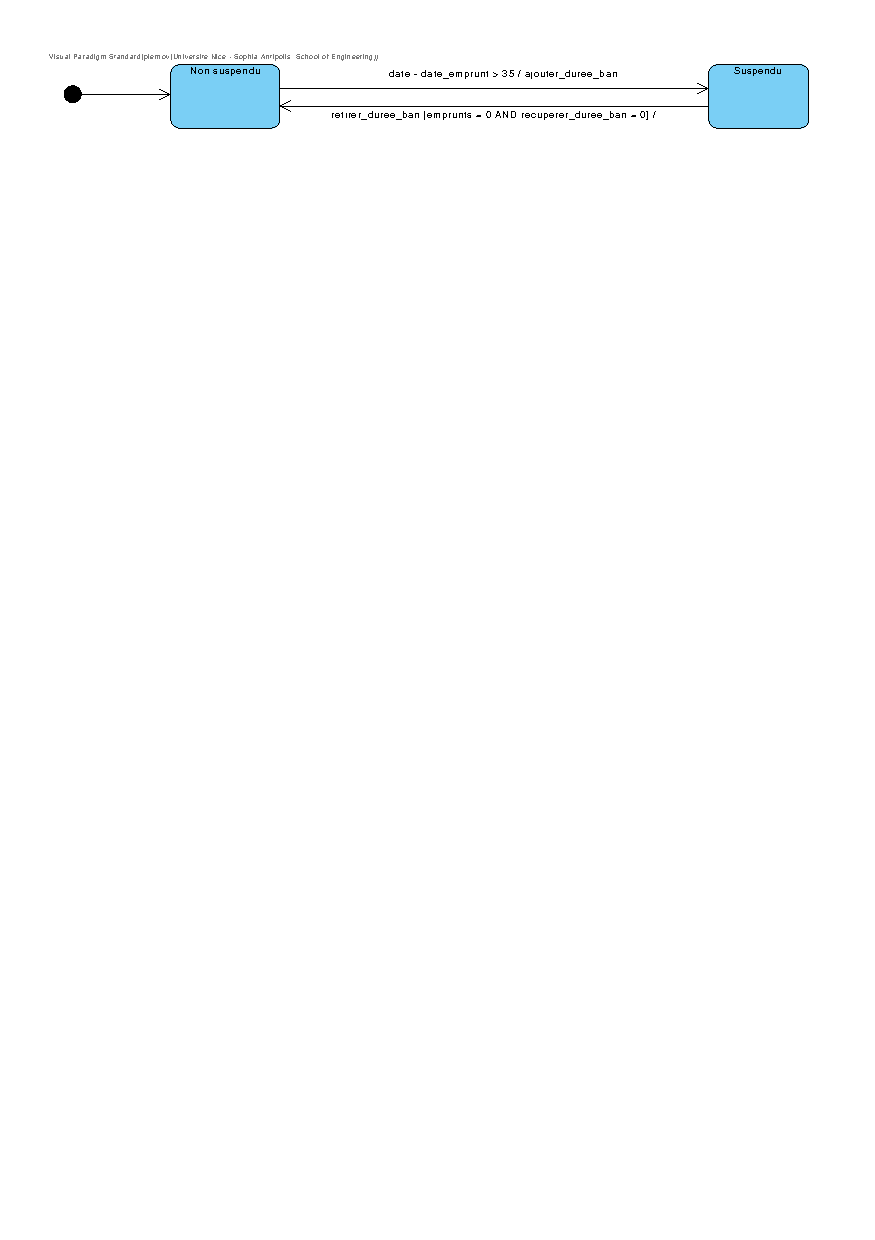
\includegraphics[scale=1.5]{state_individu}
\vspace*{-4em}

\section{Auto-évaluation}
\begin{itemize}
	\item \textbf{Cancela Joël 100pts}
		Joël a travaillé sur le diagramme des cas d'utilisation, le(s) diagrammes d'états et la rédaction du rapport.
	\item \textbf{Bounouas Nassim 100pts}
		Nassim a travaillé sur le diagramme de classe, le diagramme de séquence "Enregistrer un retour" et la rédaction du rapport.
	\item \textbf{Mortara Johann 100pts}
		Johann a travaillé sur le diagramme de séquence "Enregistrer un emprunt", le diagramme de cas d'utilisation détaillé "Enregistrer un emprunt", et le diagramme de séquence "Réserver un livre".
	\item \textbf{Novac Pierre-Emmanuel 100pts}
		Pierre-Emmanuel a travaillé sur le diagramme de classe, les diagrammes de séquence "Relancer pour rendu de livre", "Rechercher un document" et sur la rédaction du rapport.
\end{itemize}

\end{document}
